
\subsection{Cohesive laws}

\subsubsection{Snozzi-Molinari law}

\begin{figure}
  \centering
  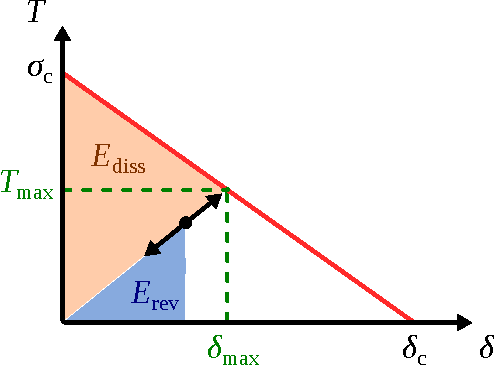
\includegraphics[width=.4\textwidth]{figures/law}
  \caption{Linear irreversible cohesive law.}
  \label{fig:smm:coh:linear_cohesive_law}
\end{figure}

The Snozzi-Molinari~\cite{snozzi_cohesive_2013} linear irreversible
cohesive law has been implemented in \akantu as
\code{material\_cohesive\_linear} (see
figure~\ref{fig:smm:coh:linear_cohesive_law}). It is an extension to
the Camacho-Ortiz~\cite{camacho_computational_1996} cohesive law in
order to make dissipated fracture energy path-dependent. The concept
of free potential energy is dropped and a new independent parameter
$\kappa$ is introduced:
\begin{equation}
  \kappa = \frac{G_\mathrm{c, II}}{G_\mathrm{c, I}}
\end{equation}
where $G_\mathrm{c, I}$ and $G_\mathrm{c, II}$ are respectively the
necessary works of separation per unit area to open completely a
cohesive zone under mode I and mode II. Their model yields to the
following equation for cohesive tractions in case of crack opening
\begin{equation}
  \label{eq:smm:coh:tractions}
  \vec{T} = \left( \frac{\beta^2}{\kappa} \Delta_\mathrm{t} \vec{t} +
    \Delta_\mathrm{n} \vec{n} \right)
  \frac{\sigma_\mathrm{c}}{\delta}
  \left( 1- \frac{\delta}{\delta_\mathrm{c}} \right)
\end{equation}
where $\sigma_\mathrm{c}$ is the material strength along the fracture,
$\delta_\mathrm{c}$ the critical effective displacement after which
cohesive tractions are zero (complete decohesion), $\Delta_\mathrm{t}$
and $\Delta_\mathrm{n}$ are respectively the tangential and normal
components of the opening displacement vector $\vec{\Delta}$. The
effective opening displacement is
\begin{equation}
  \delta = \sqrt{\frac{\beta^2}{\kappa^2} \Delta_\mathrm{t}^2 +
    \Delta_\mathrm{n}^2}
\end{equation}
In case of unloading or reloading $\delta < \delta_\mathrm{max}$,
tractions are calculated as
\begin{align}
  T_\mathrm{n} &= \Delta_\mathrm{n}\,
  \frac{\sigma_\mathrm{c}}{\delta_\mathrm{max}}
  \left( 1- \frac{\delta_\mathrm{max}}{\delta_\mathrm{c}} \right) \\
  T_\mathrm{t} &= \frac{\beta^2}{\kappa}\, \Delta_\mathrm{t}\,
  \frac{\sigma_\mathrm{c}}{\delta_\mathrm{max}}
  \left( 1- \frac{\delta_\mathrm{max}}{\delta_\mathrm{c}} \right)
\end{align}
so that they vary linearly between the origin and the maximum attained
tractions. In this law dissipated and reversible energies are
\begin{align}
  E_\mathrm{diss} &= \frac{1}{2} \sigma_\mathrm{c}\, \delta_\mathrm{max}\\[1ex]
  E_\mathrm{rev} &= \frac{1}{2} T\, \delta
\end{align}
Moreover a damage parameter $D$ can be defined as
\begin{equation}
  D = \min \left(
    \frac{\delta_\mathrm{max}}{\delta_\mathrm{c}},1 \right)
\end{equation} which varies from 0 (undamaged condition) and 1 (fully
damaged condition). This variable can only increase because damage is
an irreversible process.

\subsubsection{Cohesive elements}

Cohesive elements are a numerical tool that lets a crack propagate
along the edges of standard elements. The cohesive elements that have
been implemented in Akantu are based on the work of Ortiz and
Pandolfi~\cite{ortiz1999}.

\begin{figure}
  \centering
  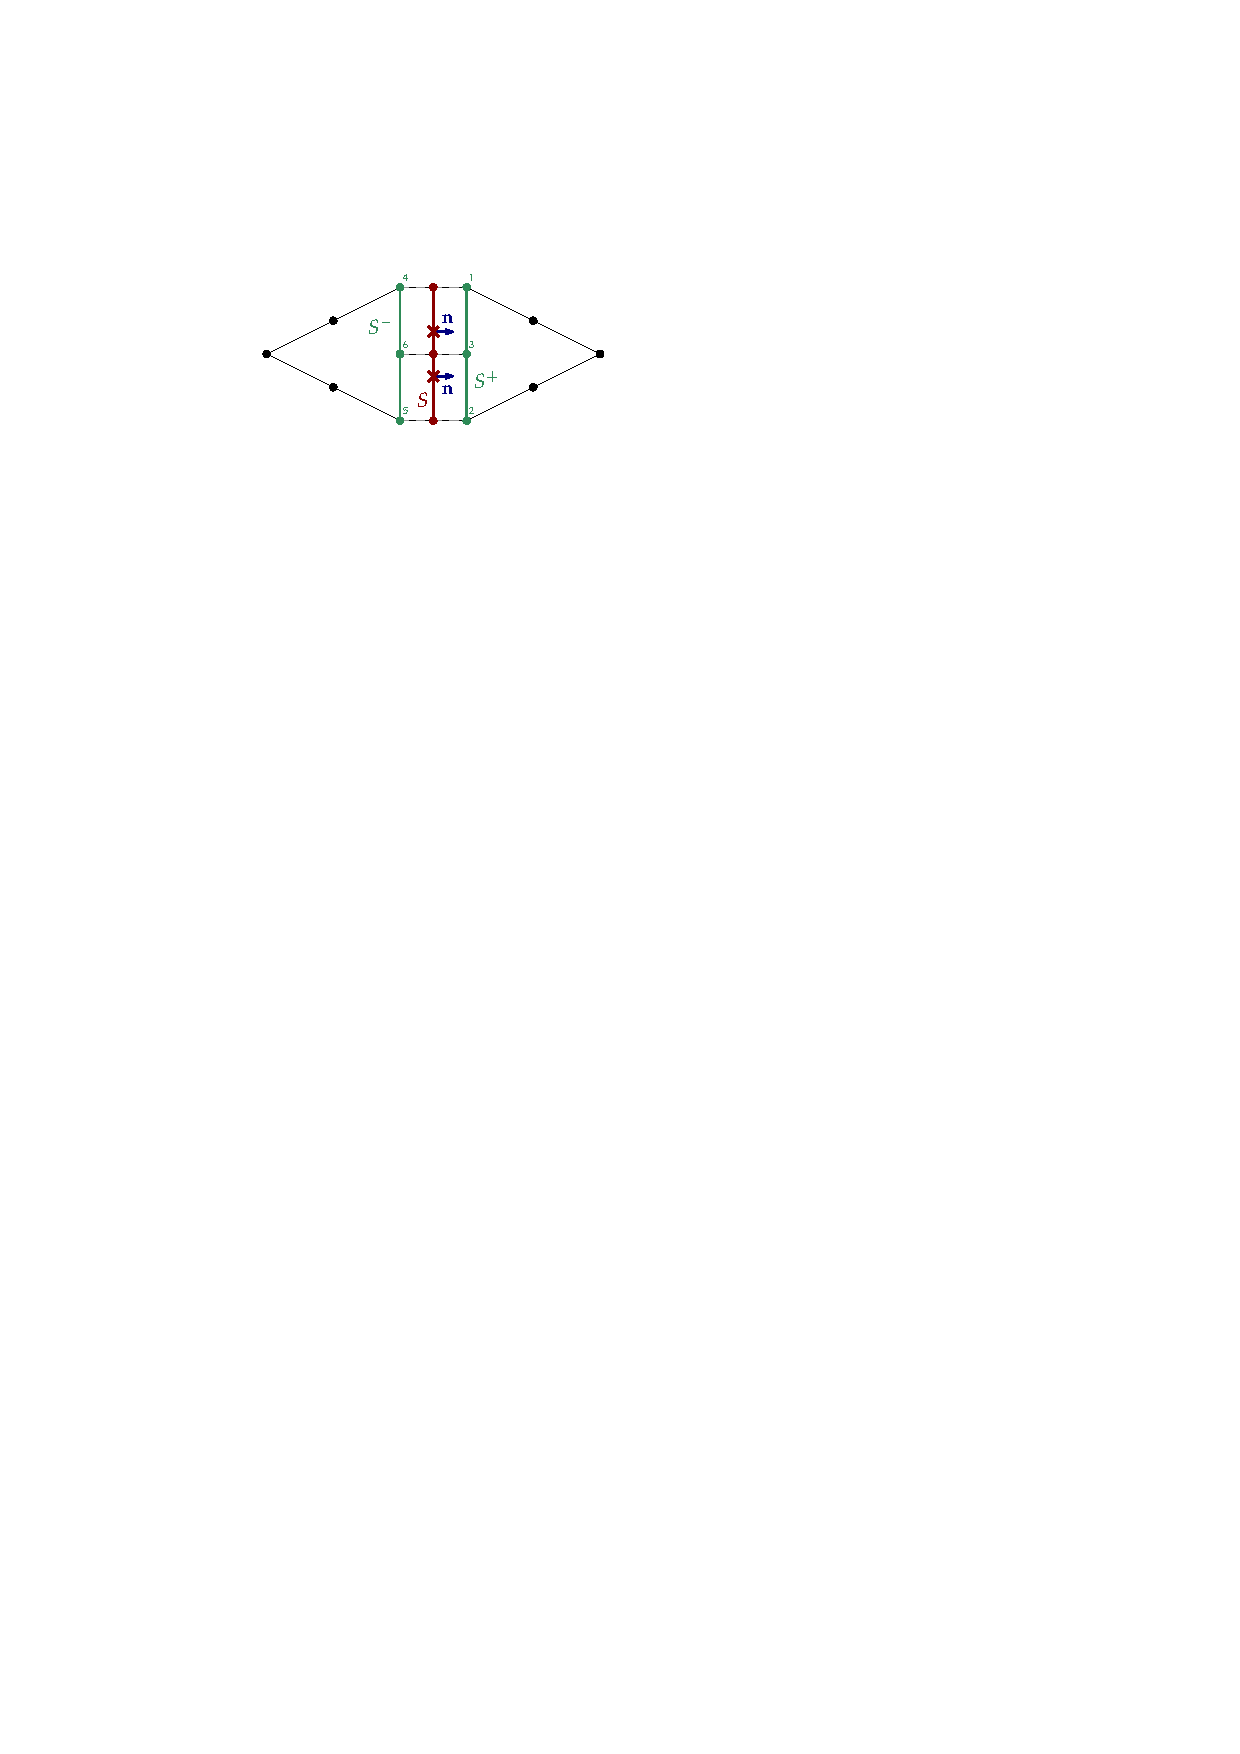
\includegraphics[width=.55\textwidth]{figures/cohesive2d}
  \caption{Cohesive element in 2D for quadratic triangular elements
    T6.}
  \label{fig:smm:coh:cohesive2d}
\end{figure}

\begin{figure}
  \centering
  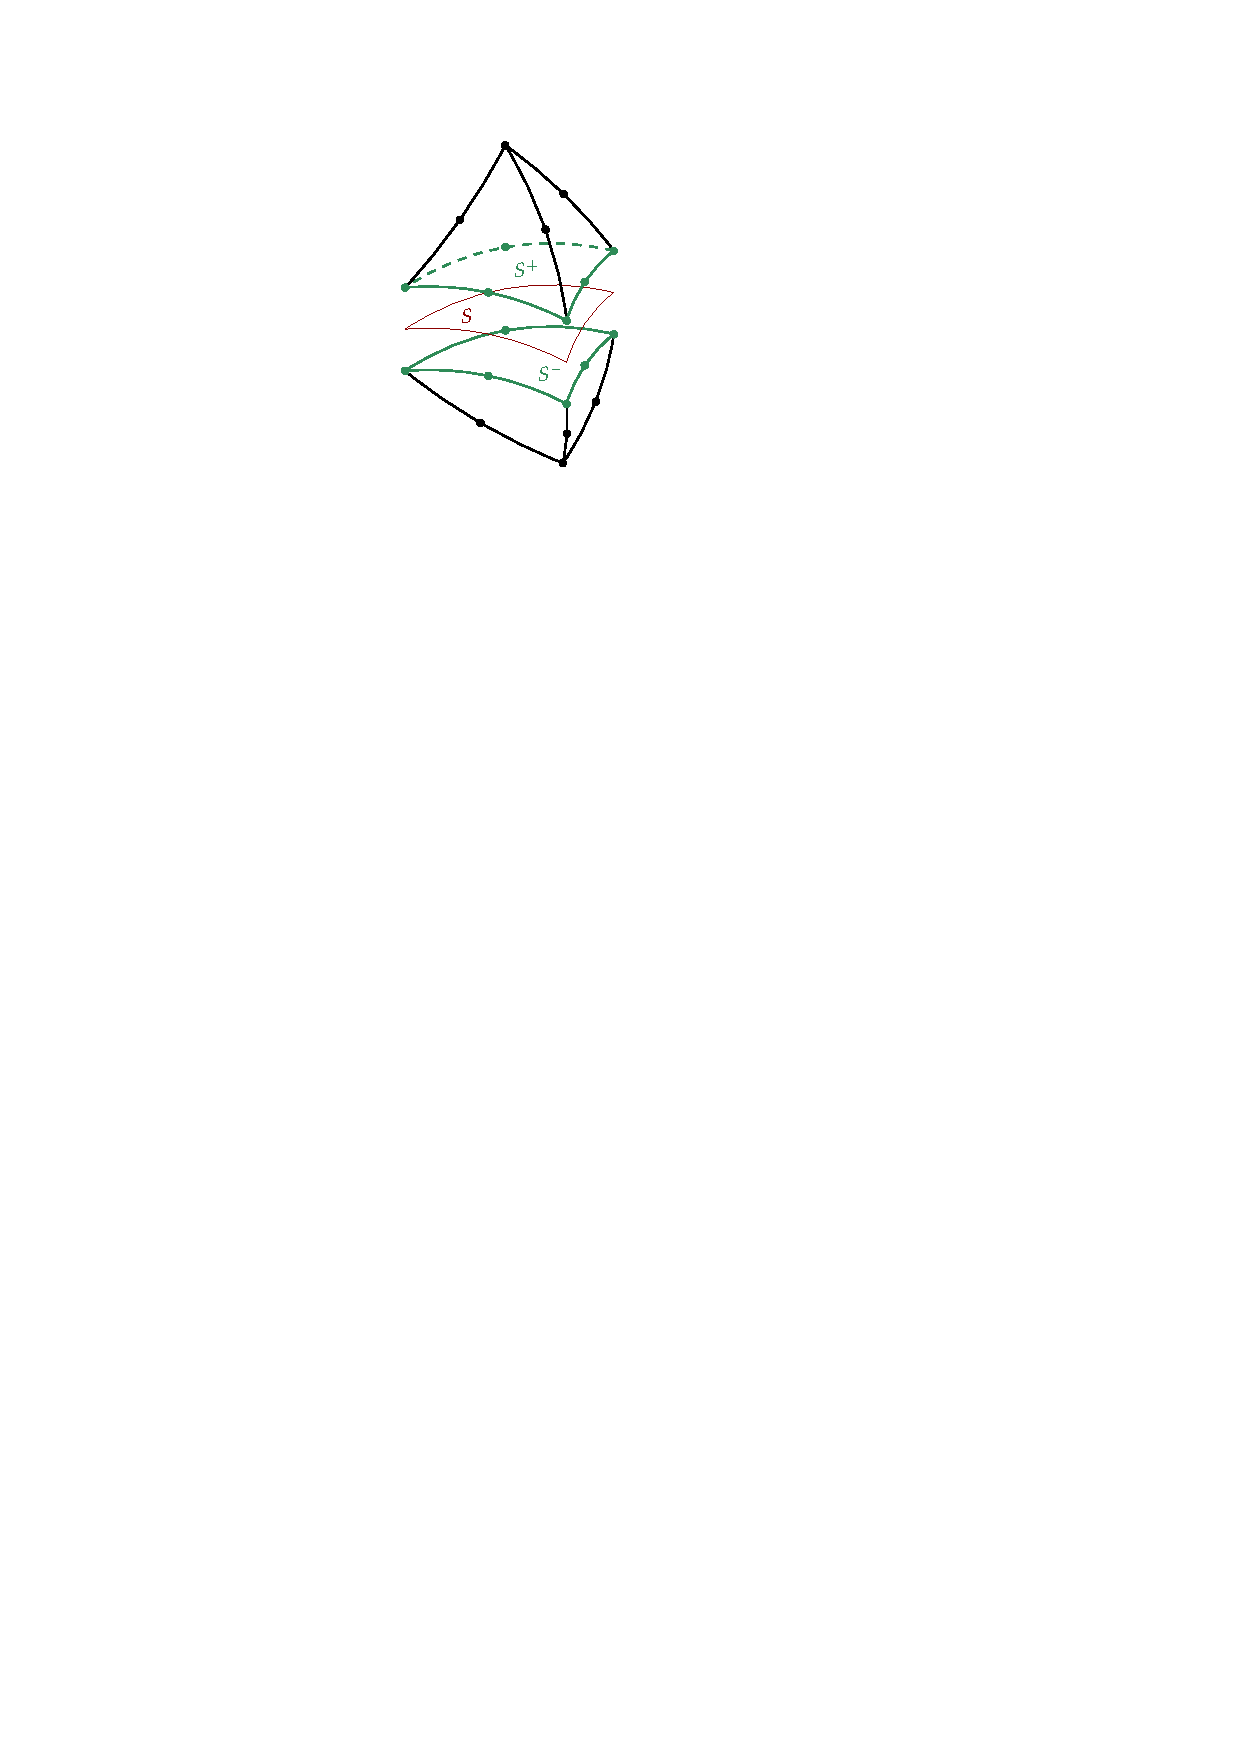
\includegraphics[width=.25\textwidth]{figures/cohesive3d}
  \caption{Cohesive element in 3D for quadratic tetrahedrons T10.}
  \label{fig:smm:coh:cohesive3d}
\end{figure}

Cohesive elements consist of a couple of surface elements which are
coincident in space when the opening displacement is zero. Two
schematics of cohesive elements in 2D and 3D can be seen in
figures~\ref{fig:smm:coh:cohesive2d}
and~\ref{fig:smm:coh:cohesive3d}. The two surface elements, denoted by
$S^-$ and $S^+$, must be of the same type and they correspond to the
facet element of the standard elements. All the computations are done
on the middle surface $S$, whose nodal coordinates are just the
average between those of $S^+$ and $S^-$.

In order to track normal and tangential openings it is convenient to
define a unique normal direction $\vec{n}$ for each quadrature point
of the cohesive element. By convention the normal points from $S^-$ to
$S^+$. The opening displacement vector is
\begin{equation}
  \label{eq:opening_displacement}
  \vec{\Delta} (\vec{s}) = \sum_{n=1}^N \llbracket \vec{x}_n \rrbracket N_n (\vec s)
\end{equation}
where $N_n$ are the shape functions of the cohesive element (they are
exactly the same of those of a single surface element) and
\begin{equation}
  \label{eq:disp_difference}
  \llbracket \vec{x}_n \rrbracket = \vec{x}_n^+ - \vec{x}_n^-
\end{equation}
in which $\vec{x}_n^\pm$ for $n=1,\dots,N$ are the current coordinates
of the nodes.

The quantities that have been defined so far are sufficient to
completely define the cohesive tractions per unit deformed
area. Indeed equation~\eqref{eq:smm:coh:tractions} can be rewritten as
\begin{equation}
  \vec{T} = \left[ \frac{\beta^2}{\kappa} \vec{\Delta} +
    \left( 1- \frac{\beta^2}{\kappa}\right)
    \left( \vec{\Delta} \cdot \vec{n}\right) \vec{n} \right]
  \frac{\sigma_\mathrm{c}}{\delta}
  \left( 1- \frac{\delta}{\delta_\mathrm{c}} \right) =
  \vec{T}(\vec{\Delta}, \vec{n})
\end{equation}
because the tangential direction $\vec{t}$ depends on the normal one
$\vec{n}$. By interpolation it is now possible to derive the nodal
forces as
\begin{equation}
  f_{in}^\pm = \mp \int_{S_0} T_i N_n\, \mathrm{d}S_0
\end{equation}
in which the integral extends over the undeformed middle surface $S_0$
of the cohesive element.

\begin{figure}
  \centering
  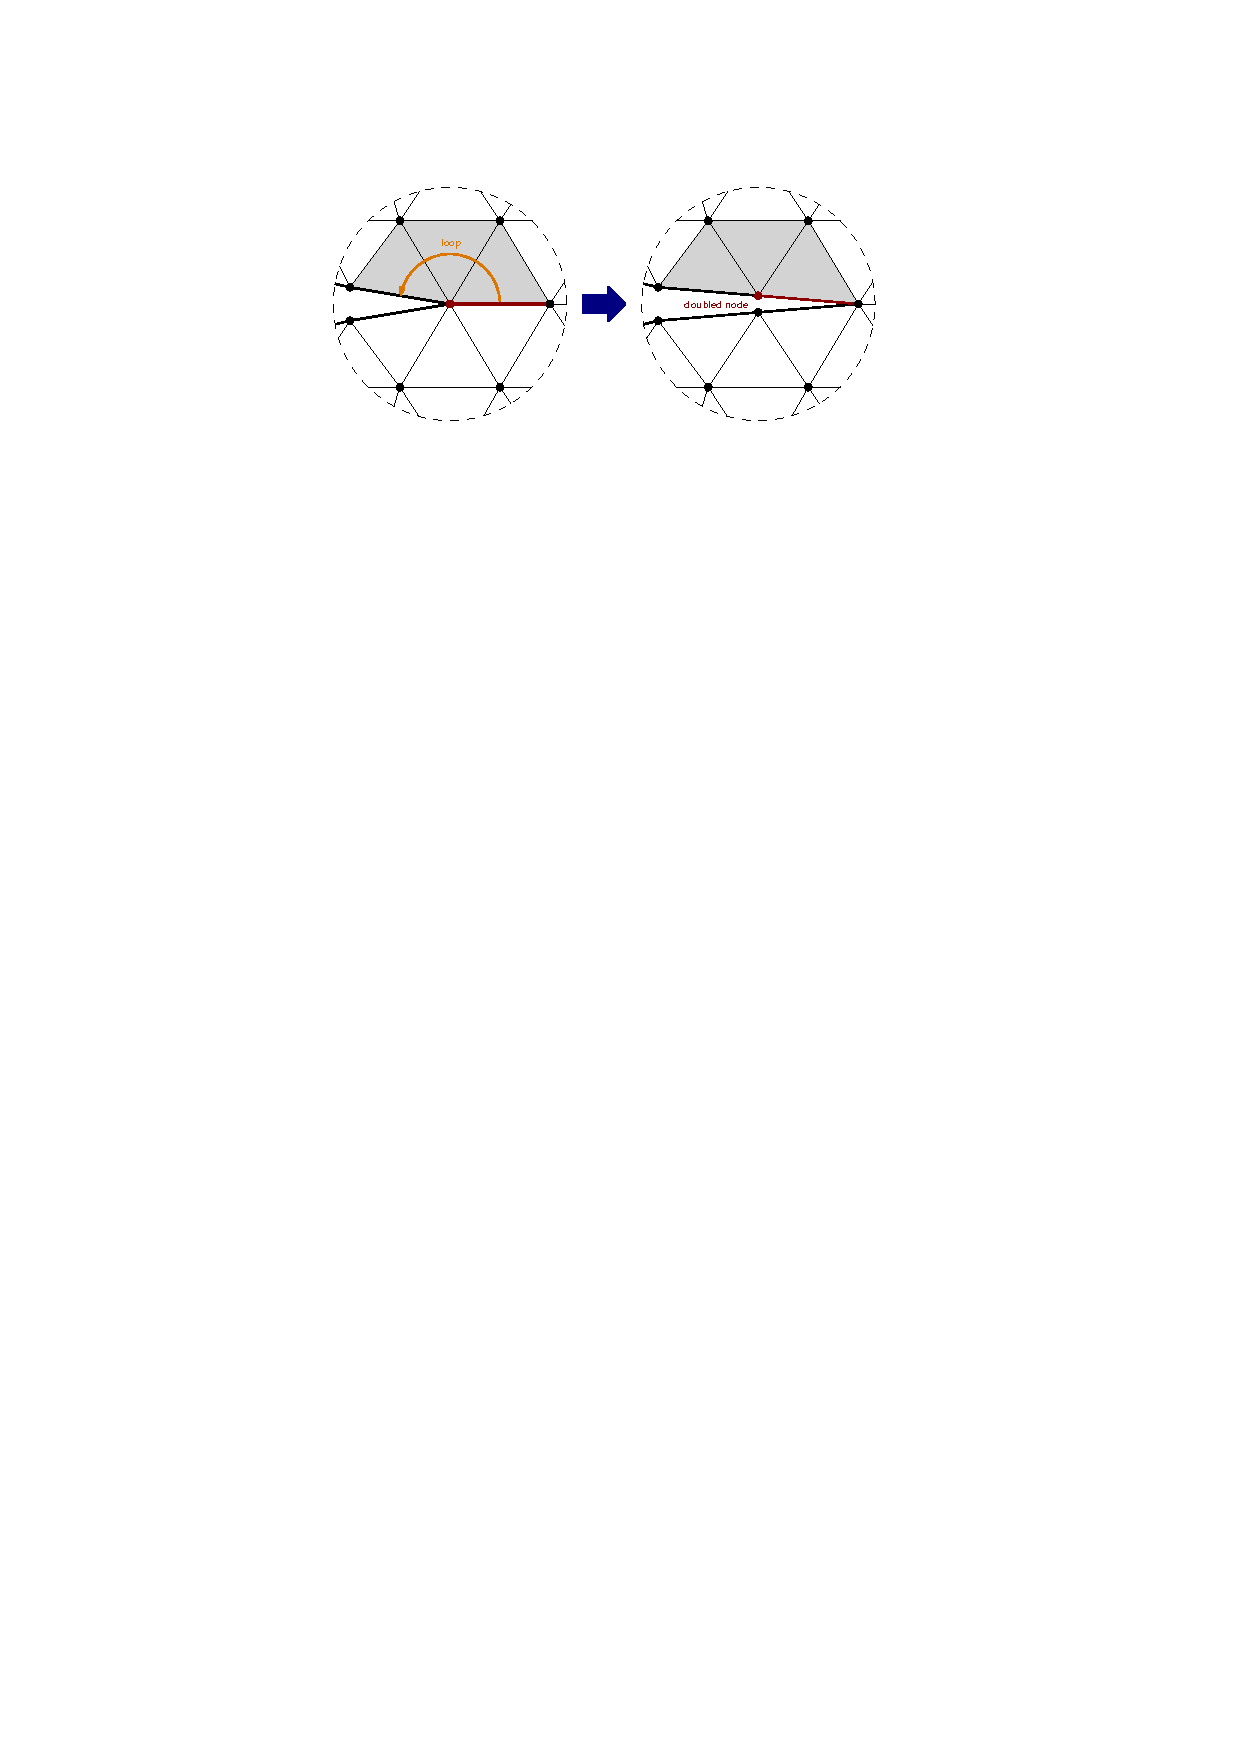
\includegraphics[width=.8\textwidth]{figures/insertion}
  \caption{Insertion of a cohesive element.}
  \label{fig:smm:coh:insertion}
\end{figure}

Cohesive element insertion can be carried out dynamically in
\akantu. More specifically, normal and tangential stresses along the
edges of standard elements are used to compute the effective stress
\begin{equation}
  \sigma_\mathrm{eff} = \sqrt{\sigma_\mathrm{n}^2 +
    \frac{\tau_\mathrm{nt}^2}{\beta^2}}
\end{equation}
where the indexes $n$ and $t$ respectively refer to normal and
tangential directions. Obviously, if $\sigma_\mathrm{n}$ is
compressive, its contribution is not considered. The so computed
effective stress $\sigma_\mathrm{eff}$ is monitored, and when it
overcomes a threshold stress on a certain edge a new cohesive element
is inserted. New nodes are added and the element connectivity is
updated (see figure~\ref{fig:smm:coh:insertion}). This topological
mesh changing technique is very convenient because it allows
simulating crack propagation without remeshing the domain.



\subsubsection{Exponential cohesive law}

Ortiz and Pandolfi proposed this cohesive law in 1999 \ref{ortiz1999}.  The
traction-opening equation for this law is as following:

\begin{equation}
  \label{eq:exponential_law}
  t = e \sigma_c \frac{\delta}{\delta_c}e^{-\delta/ \delta_c}
\end{equation}


This equation is plotted in figure (\ref{fig:smm:CL:ECL}).

 \begin{figure}[!htb]
    \begin{center}
      \includegraphics[width=0.6\textwidth,keepaspectratio=true]{figures/cohesive_exponential.pdf}
      \caption{Exponential cohesive law}
      \label{fig:smm:CL:ECL}
    \end{center}
  \end{figure}



\subsubsection{Static cohesive element}

For  the  static  analysis   of  the  structures  containing  cohesive
elements, the stiffness of the cohesive elements should also be added to the
total      stiffness       of      the      structure.      Therefore,
the  function  \code{assembleStiffnessMatrix}  is written  in  the
\code{MaterialCohesive}.

Considering a typical cohesive element as explained in figure ???, the opening
displacement along the mid-surface can be written as:

\begin{equation}
  \label{eq:opening}
  \delta(\xi) = [[\mat{u}]] \mat{N}(\xi) =
\begin{bmatrix}
u_3-u_0 & u_4-u_1 & u_5-u_2\\
v_3-v_0 & v_4-v_1 & v_5-v_2
\end{bmatrix}
\begin{bmatrix}
N_0(\xi) \\ N_1(\xi) \\ N_2(\xi)
\end{bmatrix} =
\mat{N A U}
\end{equation}

 The \mat{U} , \mat{A} and \mat{N} are as following:

\begin{equation}
  \mat{U} = \left [
\begin{array}{c c c c c c c c c c c c}
u_0 & v_0 & u_1 & v_1 & u_2 & v_2 & u_3 & v_3 & u_4 & v_4 & u_5 & v_5
\end{array}\right ]
\end{equation}


\begin{equation}
  \mat{A} = \left [\begin{array}{c c c c c c c c c c c c}
1 & 0 & 0 & 0& 0 & 0 & -1& 0 & 0 &0 &0 &0\\
0 &1& 0&0 &0 &0 &0 & -1& 0& 0 & 0 &0\\
0 &0& 1&0 &0 &0 &0 & 0& -1& 0 & 0 &0\\
0 &0& 0&1 &0 &0 &0 & 0& 0& -1 & 0 &0\\
0 &0& 0&0 &1 &0 &0 & 0& 0& 0 & -1 &0\\
0 &0& 0&0 &0 &1 &0 & 0& 0& 0 & 0 &-1
\end{array} \right ]
\end{equation}


 \begin{equation}
 \mat{N} = \begin{bmatrix}
N_0(\xi) & 0 & N_1(\xi) &0 & N_2(\xi) & 0\\
0 & N_0(\xi)& 0 &N_1(\xi)& 0 & N_2(\xi)
\end{bmatrix}
\end{equation}

The consistent stiffness matrix for the element is obtained as

\begin{equation}
  \label{eq:cohesive_stiffness}
  \mat{K}    =    \delta    \mat{U}^T    \int_{\Gamma_c}    {\mat{P}^t
    \frac{\partial{\mat{t}}} {\partial{\delta}} \mat{P} d
    \Gamma \Delta \mat{U}}
\end{equation}

In which the  tangent matrix is calculated based  on the equation \ref
{eq:tangent_cohesive} after
performing necessary derivation:

\begin{equation}
  \label{eq:tangent_cohesive}
   \frac{\partial{\mat{t}}} {\partial{\delta}} = \hat{\mat{t}} \otimes
   \frac                       {\partial{(t/\delta)}}{\partial{\delta}}
   \frac{\hat{\mat{t}}}{\delta}+ \frac{t}{\delta}  [ \beta^2 \mat{I} +
   (1-\beta^2) (\mat{n} \otimes \mat{n})]
\end{equation}

 In which $\frac{\partial{(t/\delta)}}{\partial{\delta}}$ in the first
 term is

\begin{equation}
 \frac{\partial{(t/ \delta)}}{\partial{\delta}} = \left\{\begin{array} {l l}
-e  \frac{\sigma_c}{\delta_c^2  }e^{-\delta  /  \delta_c} &  \quad  if
\delta \geq \delta_{max}\\
 0 & \quad if \delta < \delta_{max}, \delta_n > 0
\end{array} \right.
\end{equation}

This      tangent      matrix      is     implemented      in      the
\code{computeTangentStiffness} function for
the exponential law.

A full example for the static analysis of the cohesive elements can be
found in \code{\examplesdir/static\_cohesive}.




%%% Local Variables:
%%% mode: latex
%%% TeX-master: "manual"
%%% End:
